%!TEX root = TIHSC_Project_main.tex
\chapter{System Synthesis}
System synthesis is part of the model-based system design approach where it is used to obtain a transaction level model from a system specification, as seen in figure \ref{fig:modelBasedSyn}. 

\begin{figure}[H]
\centering
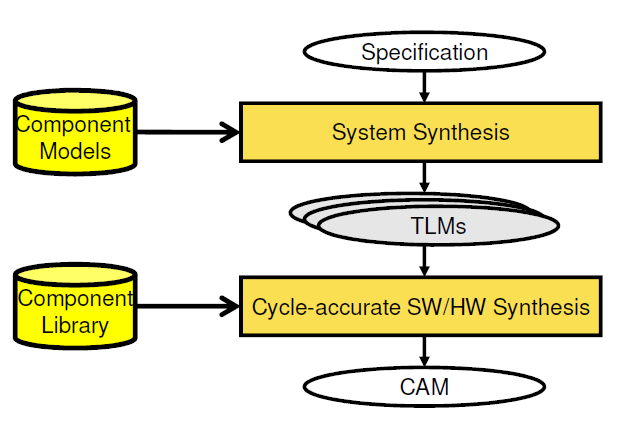
\includegraphics[scale=0.5]{modelBasedSynthesis}
\caption{Model bases synthesis}
\label{fig:modelBasedSyn}
\end{figure}

The system behavioural model in figure \ref{fig:SystemBehavioralModel} describes the specification for a Texton mapping system. 
The processes, channels and memory variables from the specification model is used as input to the different steps of the system synthesis.  

\section{Allocation}
The first step of system synthesis is allocation of the needed hardware components. 
The processes of the specification model suggest the need for at least one CPU to handle reading and writing of the image. 
All the processes could be run on a single CPU, however given requirement \ref{req:timeReq} which states that the Texton filtering should be done within a minute, is it unlikely that a single CPU can make it in time. 
Therefore a hardware IP block is allocated to support the CPU with the computation-heavy processes.
\\Figure \ref{fig:SystemBehavioralModel} also shows that processes P2 and P3 depend on a memory variable, which is allocated as a memory component. The allocated components are shown in figure \ref{fig:allocHardComps}.

\begin{figure}[H]
\centering
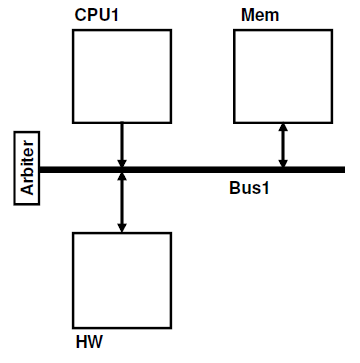
\includegraphics[scale=0.5]{Allocating}
\caption{Allocated hardware components}
\label{fig:allocHardComps}
\end{figure}


\section{Mapping}

Overall three alternative bindings have been considered. The first alternative is illustrated in Figure ~\ref{fig:Binding1}. Here every process is placed in software (CPU). This model will be the fastest to develop and probably the cheapest. However by placing the operation heavy process "K-means" in software it will probably be hard to meet the time requirement.The second alternative is illustrated in Figure ~\ref{fig:Binding2}. In this alternative every process is binded to hardware blocks. This will decrease the execution time but the implementation will also be much more complex.

\begin{figure}[H]
\centering
\begin{subfigure}{.5\textwidth}
	\centering
	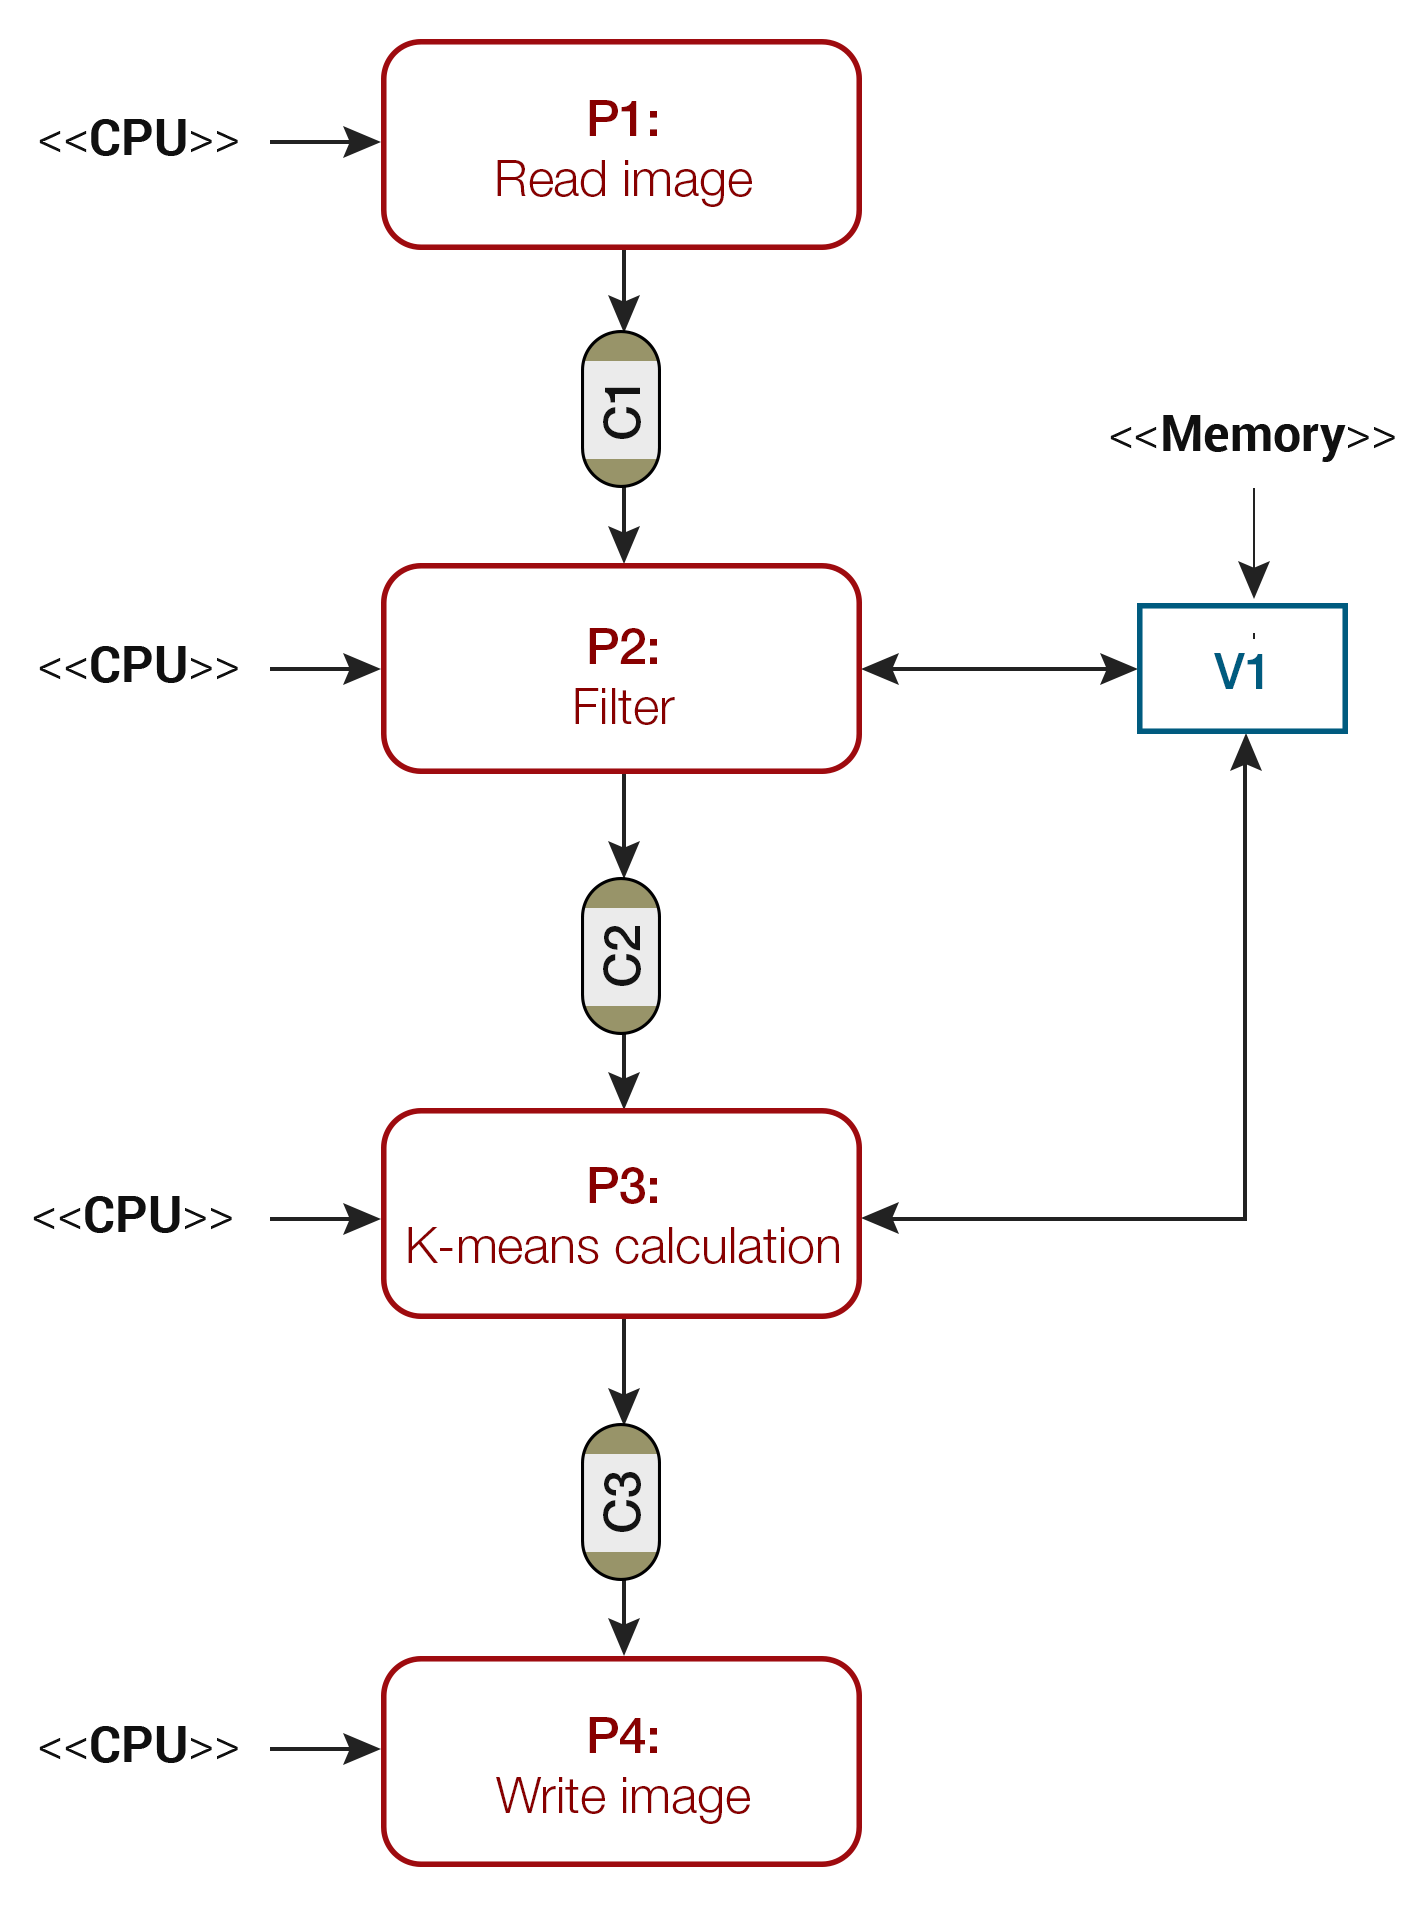
\includegraphics[width = 180 pt]{Binding1}
	\caption{1st alternative of binding - Everything in software}
	\label{fig:Binding1}
\end{subfigure}%
\begin{subfigure}{.5\textwidth}
	\centering
	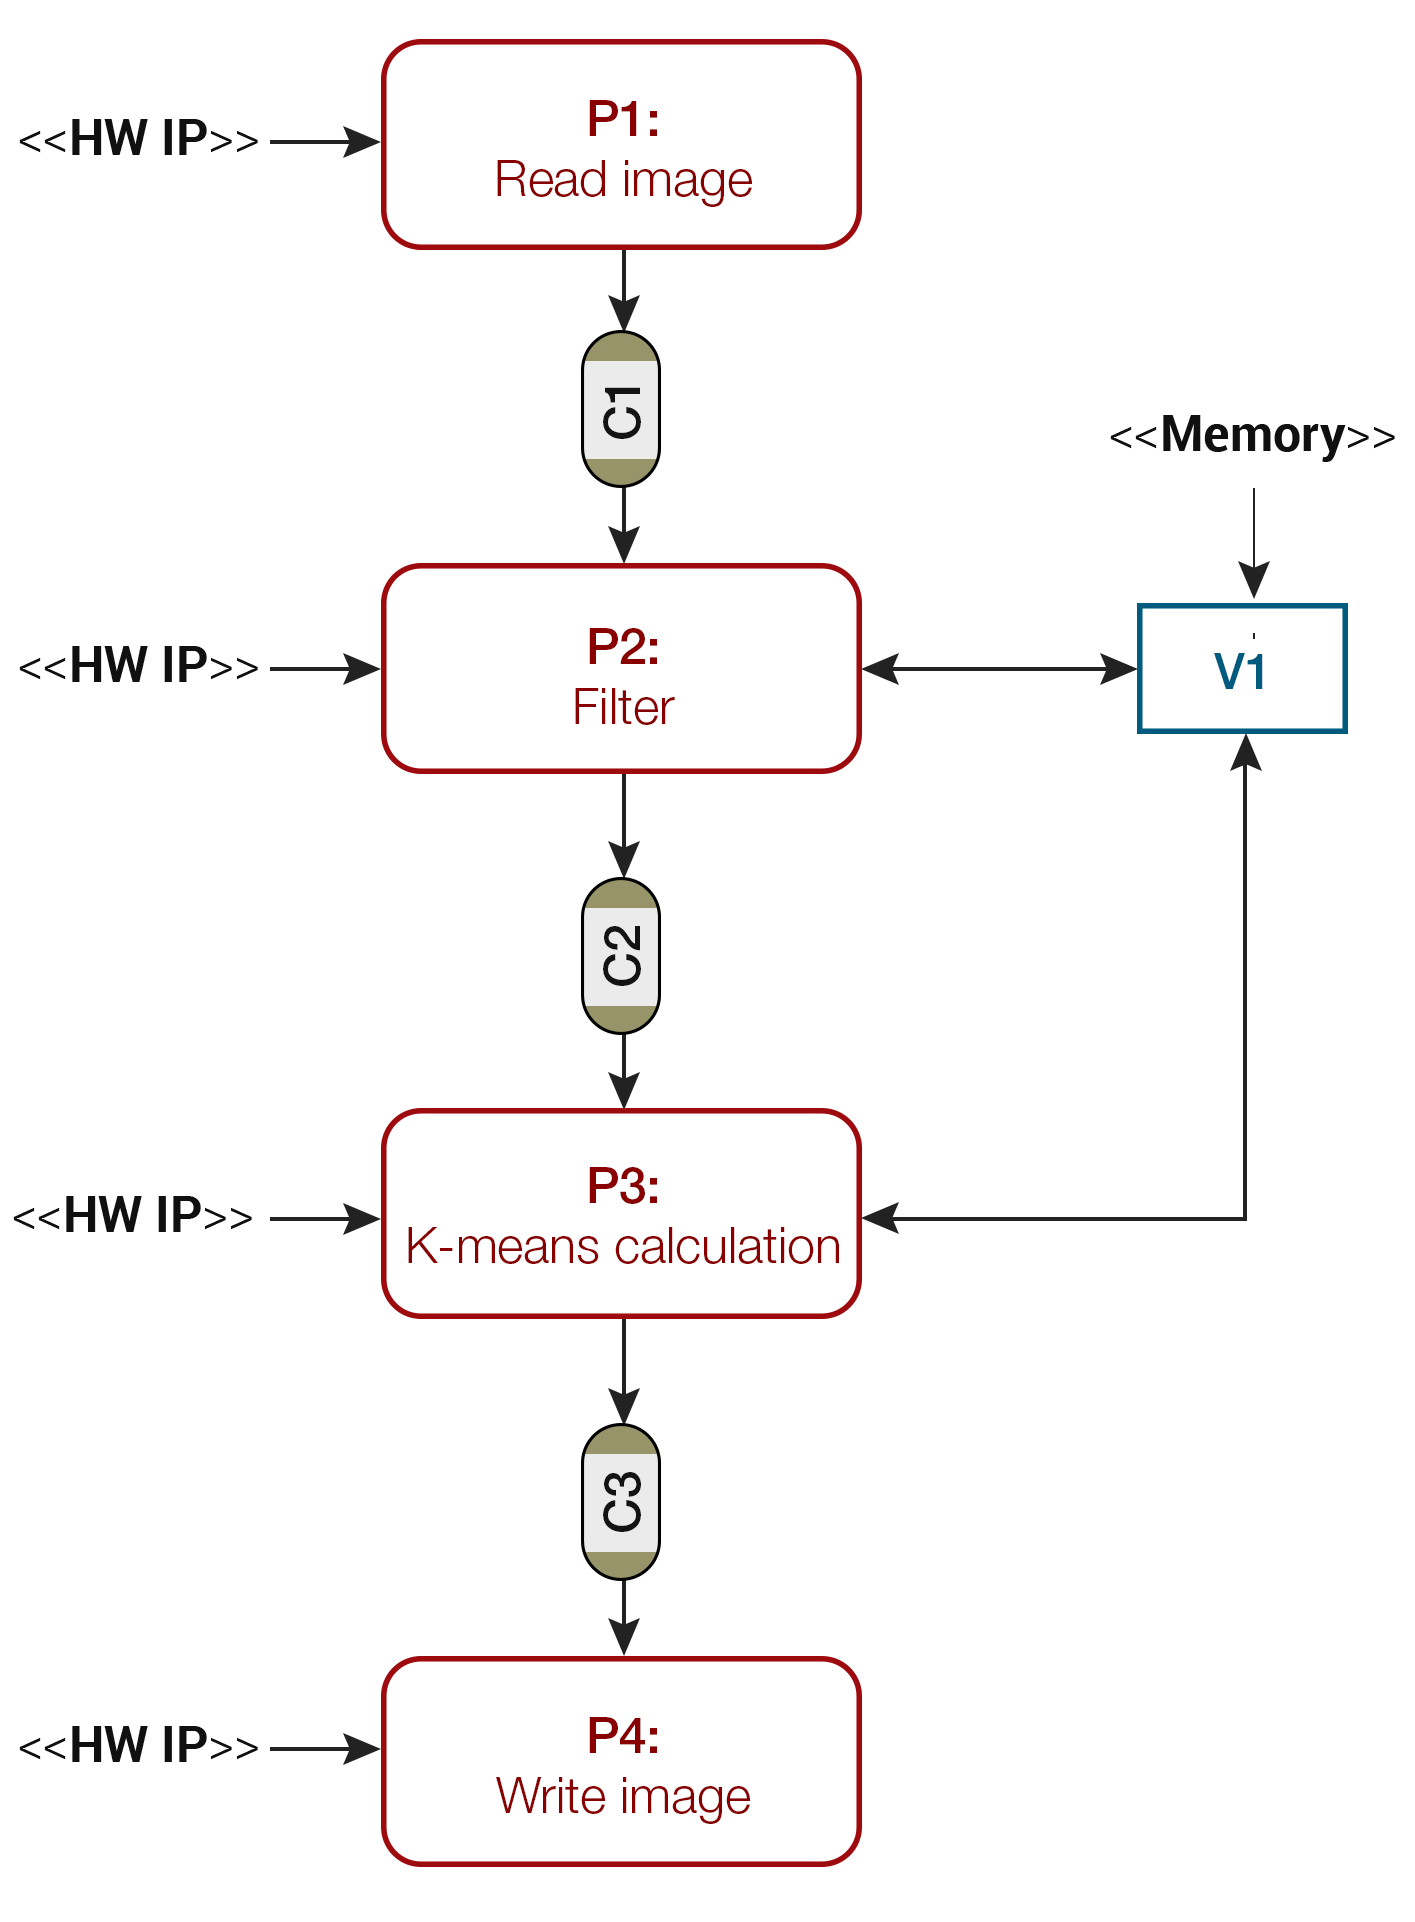
\includegraphics[width = 180 pt]{Binding2}
	\caption{2nd alternative of binding - Everything in hardware}
	\label{fig:Binding2}
\end{subfigure}%
\end{figure}

The third alternative is illustrated in Figure ~\ref{fig:Binding3}. In this alternative a combination of hardware and software is used. The reading and writing of the image is placed in software due to simplicity of these processes. The filtering process has a limited number of operation and it is estimated that it would not benefit to make this in hardware due to the added complexity compared with a minimal decrease in execution time. The most operation heavy process is the K-means calculation and paralization of this process would be highly beneficial.

\begin{figure}[H]
	\centering
	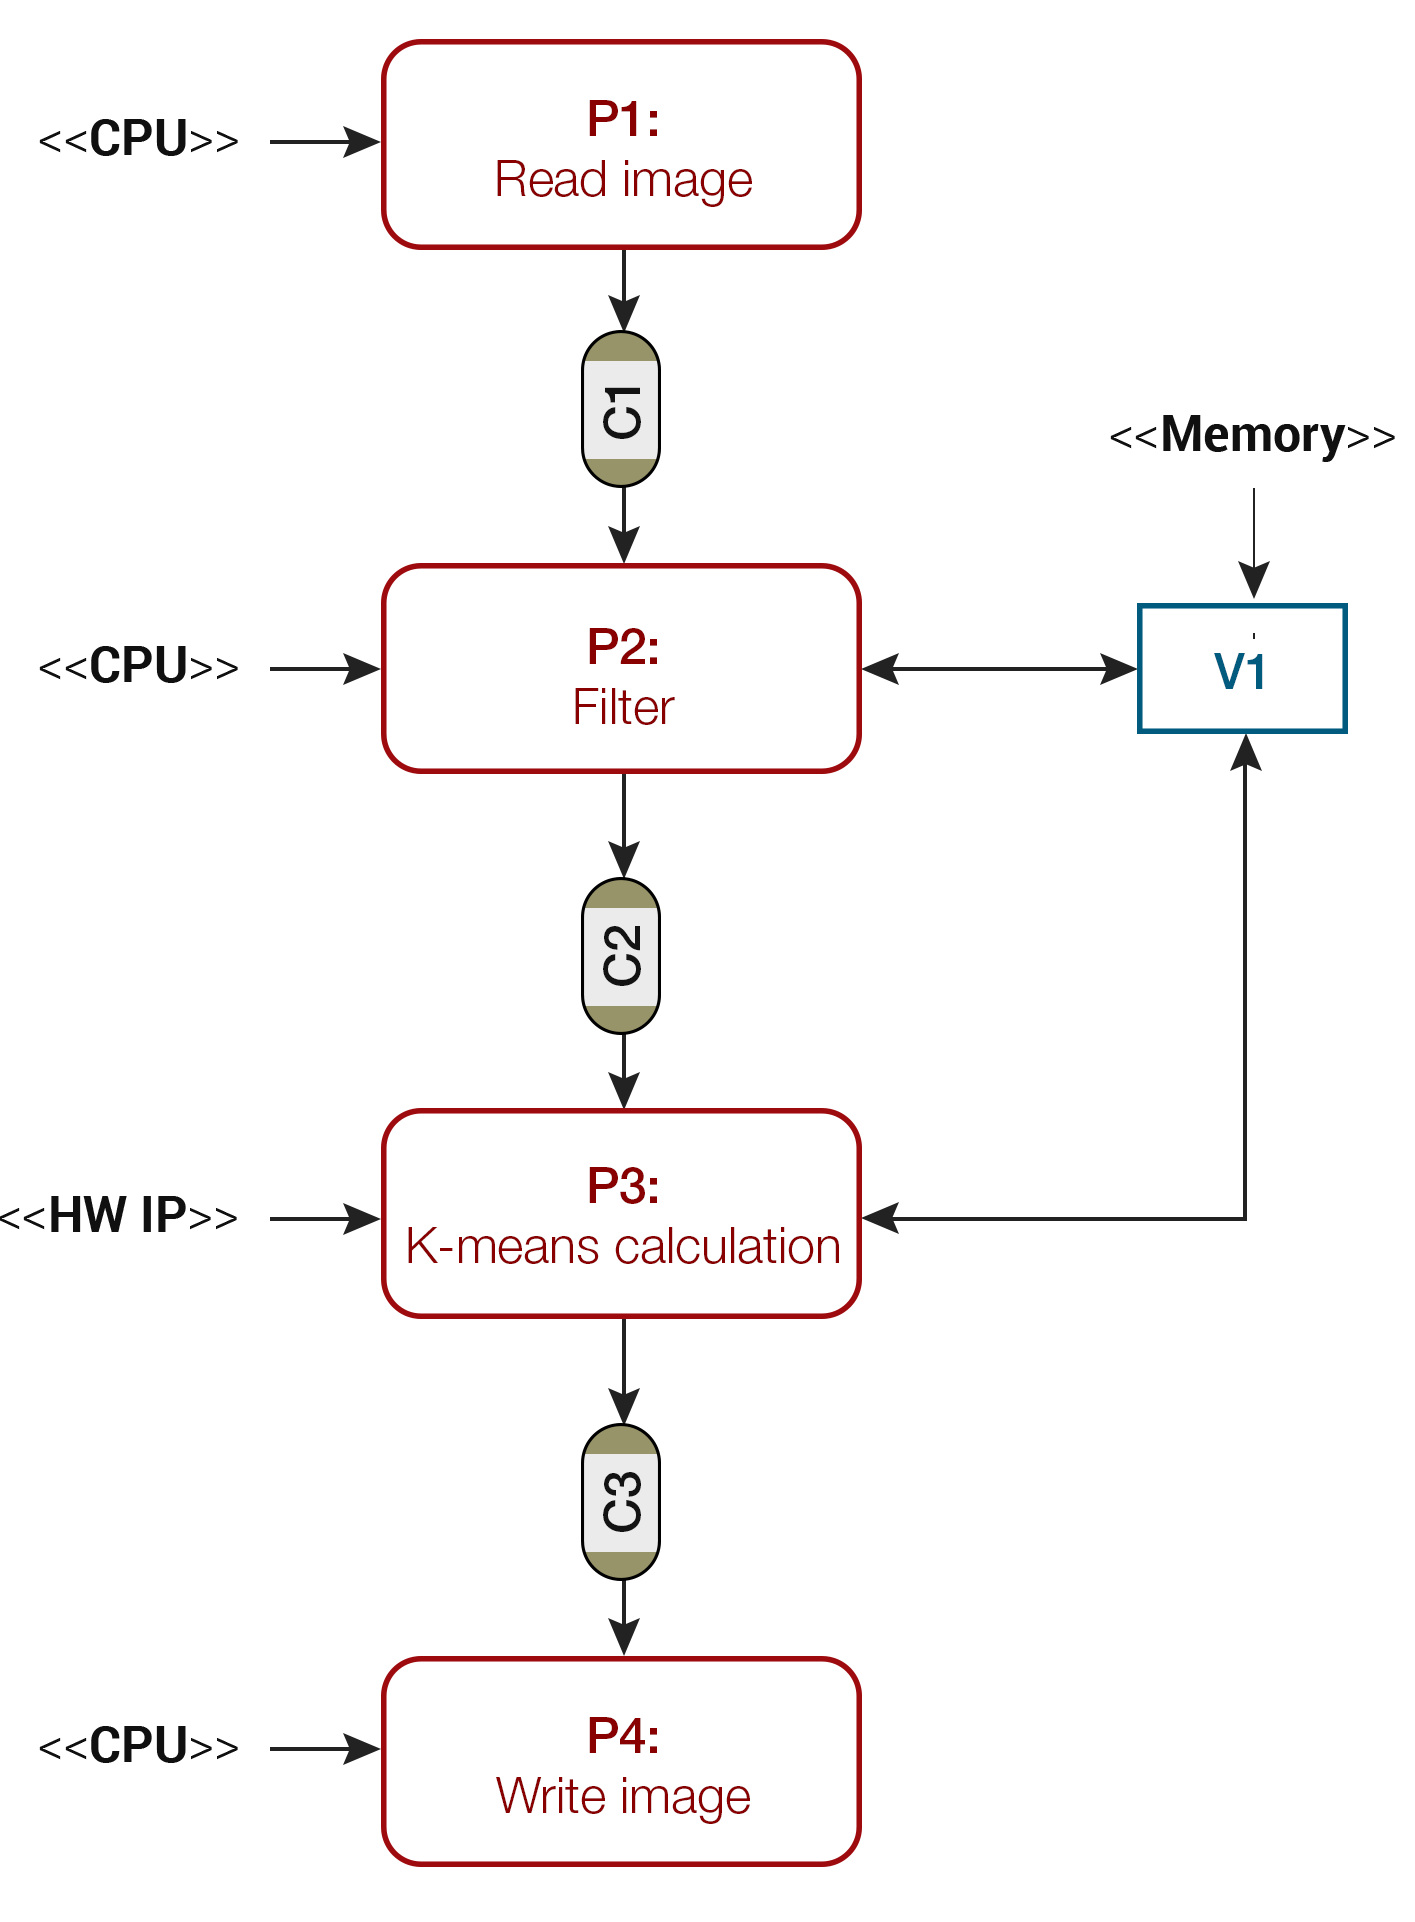
\includegraphics[width = 180 pt]{Binding3}
	\caption{3rd alternative of binding - Combination of hardware and software}
	\label{fig:Binding3}
\end{figure}

Because only one process is binded to each processing element there are no need for scheduling in this system.